% ICLR full-width figure; requires graphicx.
\begin{figure*}[t]
  \centering
  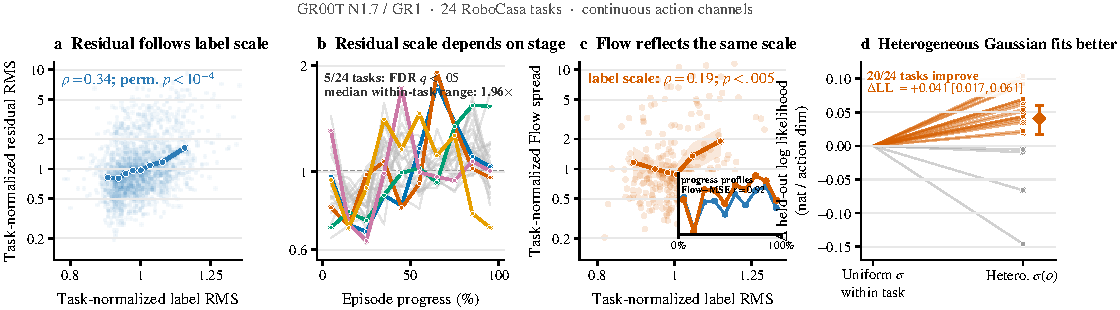
\includegraphics[width=\textwidth]{analysis/paper/heterogeneous_scale_probe/fig_heterogeneous_scale.pdf}
  \caption{\textbf{Robot-policy residuals have input-dependent scale.}
  We analyze the continuous action channels of GR00T N1.7 on 24 RoboCasa-GR1
  tasks. (a) Across 2,880 policy-held-out states, the RMS residual of a
  converged MSE policy increases with the action-label RMS after within-task
  normalization ($\rho=0.34$; within-task permutation $p<10^{-4}$).
  (b) Each curve traces residual scale over progress within one task. The five
  colored tasks retain a stage effect after Benjamini--Hochberg correction
  ($q<.05$); the other 19 tasks are shown in gray. The median within-task
  max/min scale ratio is $1.96\times$. (c) At 240 matched inputs, we sample
  32 action chunks from Flow and define spread as their RMS deviation from the
  sample mean. Flow spread correlates with label scale ($\rho=0.19$,
  $p<.005$), and its progress profile closely tracks the MSE residual profile
  ($r=0.92$). (d) Keeping the action mean fixed, a cross-fitted Gaussian with
  input-dependent scale attains higher held-out log likelihood than one with
  uniform scale within each task on 20 of 24 tasks ($+0.041$ nat per action
  dimension; 95\% task-bootstrap CI $[0.017,0.061]$). Together, these results
  motivate heteroscedastic regression.}
  \label{fig:heterogeneous-scale}
\end{figure*}
